\documentclass[a4paper,11pt,numreferences,mathsec,kaplist]{isuepsutf8}
\usepackage{isuutf8}
\usepackage{accents}
\usepackage{caption}

\begin{document}
\setcounter{aqwe}{1} % Если статья на английском языке, то значение счетчика aqwe установить равным 2
\begin{article}
\begin{opening}

\mytype{Научная статья}
\udk{518.517}
\msc{03C07, 03C60}%Mathematics Subject Classification

\title{Эффективный метод динамических расчетов элементов
теплоэнергетических установок, сводящий решение систем
дифференциальных уравнений в частных производных к решению задач
линейного программирования}

\author{
    А.\,М.\,Клер\spisokworks{1},
    \corrauthor{Д.\,В.\,Апанович\spisokworks{1}}
}

\institute{
    \workinsttt{1}{Институт систем энергетики им. Л.А. Мелентьева СО
    РАН, Иркутск, 664033, Российская Федерация}
\mailcorauth{dvapan@gmail.com}%адрес для переписки
}

%Информация для содержание
\avtogl{А.\,М.\,Клер, Д.\,В.\,Апанович}{Эффективный метод динамических
расчетов элементов теплоэнергетических установок, сводящий решение
систем дифференциальных уравнений в частных производных к решению
задач линейного программирования}
%на английском языке
\avtogle{A.\,Kler, D.\,Apanovich}{Efficient method of dynamic element
calculations thermal power plants, which reduces the solution of
systems of differential equations in partial derivatives to the
solution of linear programming problems}

\runningtitle{ЭФФЕКТИВНЫЙ МЕТОД ДИНАМИЧЕСКИХ РАСЧЕТОВ ЭЛЕМЕНТОВ ТЭУ}
\runningauthor{А.\,М.\,КЛЕР, Д.\,В.\,АПАНОВИЧ}

\abstractt{Расчеты динамических процессов в элементах
теплоэнергетических установок (теплообменники, камеры сгорания,
турбомашины и др.) необходимы для обоснования допустимых и оптимальных
режимов работы, выбора элементов конструктивных характеристик, оценки
их надежности и т. д. эти задачи сводятся к решению систем уравнений в
частных производных. В настоящее время для таких расчетов в основном
используются метод конечных разностей и метод конечных элементов. Эти
методы громоздки и сложны. В статье предлагается метод, основная идея
которого заключается в сведении решения указанных систем уравнений к
решению задач линейного программирования (ЛП). Работа метода
демонстрируется на примере теплообменника периодического действия. }

\keywords{численные методы, линейное программирование,
дифференциальные уравнения в частных производных, динамические
процессы}

\mythanks{Работа выполнена при финансовой
	поддержке РФФИ  (проект 00--00--00000).}

\forcitat{А.\,М.\,Клер, Д.\,В.\,Апанович}{Эффективный метод динамических
расчетов элементов теплоэнергетических установок, сводящий решение
систем дифференциальных уравнений в частных производных к решению
задач линейного программирования}

\mytypeothe{Research article}

\naze{Efficient method of dynamic element
calculations thermal power plants, which reduces the solution of
systems of differential equations in partial derivatives to the
solution of linear programming problems}

\avtore{
    A.\,M.\,Kler\spisokworks{1},
    \corrauthor{D.\,V.\,Apanovich\spisokworks{1}}
}

\inst{
    \workinsttt{1}{Melentiev Energy Systems Institute SB RAS,
    Irkutsk, 664033, Russian Federation}
\mailcorauth{dvapan@gmail.com}%адрес для переписки
}

\myastractt{Calculations of dynamic processes in elements thermal
power plants (heat exchangers, combustion chambers, turbomachines,
etc.) are necessary to justify acceptable and optimal operating modes,
select elements of structural characteristics, assess their
reliability, etc. These problems are reduced to solving systems of
equations in partial derivatives. Currently, for such calculations,
the finite difference method and the finite element method are mainly
used. These methods are cumbersome and complicated. The article
proposes a method, the main idea which is to reduce the solution of
these systems of equations to the solution of linear programming (LP)
problems. The operation of the method is demonstrated on the example
of a batch heat exchanger.}

\keywordse{numerical methods, linear programming, partial differential
equations, dynamic process} 

\mythankse{The study was financially supported by the Russian
Foundation for Basic Research (Project No. ).}


\forcitate{A.\,Kler, D.\,Apanovich}{Efficient method of dynamic
element calculations thermal power plants, which reduces the solution
of systems of differential equations in partial derivatives to the
solution of linear programming problems}

\end{opening}

\section{Введение} 

Расчеты стационарных и нестационарных режимов работы ряда элементов
теплоэнергетических установок (теплообменников различных типов, топок,
камер сгорания, турбинных ступеней и др.) сводятся к решению систем
дифференциальных уравнений в частных производных (СДУЧП). Основными
методами решения таких систем являются методы конечных разностей (МКР),
методы контрольных объемов (МКО) и методы конечных элементов (МКЭ).  

При использовании МКР на расчетной области строится сетка и для
каждого ее узла, на основе исходных дифференциальных уравнений,
формируется подсистема алгебраических уравнений
\cite{SN1978,C2020,S1985,KD2018}. В этих уравнениях частные
производные заменяются соответствующими конечными разностями.
Подсистемы алгебраических уравнений отдельных узлов сетки объединяются
в единую систему алгебраических уравнений, к которой добавляются
краевые условия. Следует отметить, что при этом точность решения СДУЧП
сильно зависит от величин шагов сетки по пространственным координатам
и по времени. Стремление поднять точность решения приводит к
сокращению размеров шагов и соответственно к увеличению числа узлов
сетки и размерности системы алгебраических уравнений. Во многих
случаях эта размерность становится столь большой, что система не может
быть решена как единое целое без использования тех или иных методов
декомпозиции.  Снижения размерности системы можно добиться
использованием сетки с переменными шагами, но это сильно усложняет
алгоритм решения задачи, что особенно ощутимо для расчетного
пространства со сложной геометрией.

МКО применим к задачам, в которых дифференциальные уравнения отражают
законы сохранения массы (полной или отдельных химических элементов),
энергии и импульса \cite{C2020,KD2018,PS1968}). К таким задачам
относится большинство задач тепломассообмена.  Поэтому данный метод
наиболее широко используется в вычислительной гидрогазодинамике. В
соответствии с МКО расчетная область разбивается на контрольные
объемы, для которых допустима неправильная геометрическая форма.  Для
каждого объема формируются балансовые уравнения, учитывающие обмен
данного объема с соседними объемами массой, энергией и импульсом. Эти
уравнения являются алгебраическими, в которых производные заменяются
на конечные разности, определяемые по значениям соответствующих
параметров в геометрических центрах смежных контрольных объемов. Кроме
того в уравнения входят площади граничных поверхностей между смежными
контрольными объемами. Причем балансы массы, энергии и импульса
соблюдаются для контрольных объемов вне зависимости от места
расположения разделяющих смежные объемы поверхностей. МКО позволяют
более точно и более просто чем МКР представить сложную расчетную
область.  К недостаткам как МКР, так и МКО следует отнести
невозможность расчета искомых переменных в точках, не являющихся
узлами сетки или центрами контрольных объемов.

МКЭ первоначально предназначались для статических расчетов
строительных конструкций \cite{CTO2018,ZTZ2005,EGH2000}. Они основаны
на разбиении расчетной области на достаточно большое число конечных
элементов простой формы, как правило, многогранников.  На каждом
элементе выделяются узлы. В первую очередь это вершины многогранников,
однако, возможен выбор в качестве узлов и других точек. Для каждого
элемента для всех искомых из системы дифференциальных уравнений
функций ищутся линейные комбинации заранее заданных базисных функций,
связывающие пространственные координаты и время с соответствующей
искомой переменной. Совокупность таких комбинаций для всех элементов
должна отвечать следующим условиям: достигается минимум суммы
квадратов невязок для всех узлов всех конечных элементов (невязки
получаются при подстановке в дифференциальные уравнения нужных
производных соответствующих линейных комбинаций базисных функций);
равенство искомых переменных в вершинах смежных элементов при
определении их из линейных комбинаций базисных функций этих элементов;
равенство расчетных краевых условий при определении их на основе
соответствующих линейных комбинаций базисных функций. Следует
отметить, что при согласованном подборе числа конечных элементов,
числа узлов в элементах и числа базисных функций можно добиться того,
что невязки в узлах элементов при соблюдении указанных условий
окажутся равными нулю, т.е. минимума достигает сумма квадратов
невязок.  При этом количество невязок должно быть равно количеству
искомых коэффициентов линейных разложений базисных функций.  Указанные
условия порождают систему алгебраических уравнений, решение которой
дает линейные комбинации базисных функций, позволяющие определить
искомые переменные в любой точке расчетной области, что является
несомненным достоинством МКЭ. Следует отметить, что если исходная
СДУЧП линейная, то и системы алгебраических уравнений, к которым
сводится приближенное решение СДУЧП, будут линейным.

При решении многих нестационарных задач с использованием МКР, МКО и
МКЭ получающиеся системы алгебраических уравнений становятся
чрезвычайно большими и для их решения используются методы
декомпозиции, состоящие, как правило, в разделении решения по
пространственным координатам и по времени.  Выделяется подсистема
уравнений, относящаяся к одному моменту времени.  После ее решения
находятся частные производные искомых величин по времени.  С
использованием этих производных определяются значения соответствующих
величин в следующий момент времени (на следующем временном слое). При
этом используются различные явные и неявные разностные схемы
\cite{J2012}.

В рассмотренных методах условием малого отклонения приближенного решения
СДУЧП от ее точного решения является малость величин характерных
геометрических размеров (шаги сетки, максимальные размеры контрольных
объемов и конечных элементов). Наиболее обоснованным численным критерием
такого отклонения (качества приближенного решения) является значение
максимальной по модулю невязки во всех рассматриваемых (контрольных) точках
расчетной области. Однако ни в одном из рассмотренных методов данный
критерий не используется. 

С учетом указанных недостатков МКР, МКО и МКЭ предлагается более
эффективный метод решения СДУЧП. Он основан на поиске таких значений
коэффициентов линейных разложений базисных функций, представляющих
зависимости искомых из СДУЧП функций от пространственных координат и
времени, при которых минимального значения достигает максимальная по модулю
невязка, определяемая среди всех невязок в заданных контрольных точках
расчетной области. Переход от минимизации суммы квадратов невязок к
минимизации максимальной по модулю невязки значительно улучшает качество
приближенного решения и позволяет перейти от малых конечных элементов к
достаточно крупным блокам, в пределах каждого из которых ищутся свои
линейные разложения базисных функций. В основе метода лежит назначение в
пределах расчетной области контрольных точек, в каждой из которых
определяются невязки. Важно подчеркнуть, что количество невязок может
и должно быть больше, причем существенно, числа коэффициентов линейных
разложений базисных функций.

Все контрольные точки расчетной области делятся на три группы. Первая
группа — это внутренние контрольные точки блоков. В данных точках
рассчитываются только невязки исходных дифференциальных уравнений,
получающиеся после подстановки в них искомых функций и их частных
производных, определяемых из линейных разложений базисных функций. Вторая
группа — это точки, лежащие на границах блоков. В этих точках невязки
дифференциальных уравнений рассчитываются для каждого смежного блока с
использованием его линейных разложений. Кроме того определяются невязки
между искомыми функциями смежных блоков. К третьей группе относятся
контрольные точки, лежащие на границах расчетной области. В этих точках
состав невязок дифференциальных уравнений дополняется невязками,
определяющими точность приближения полученного решения к начальным и
граничным условиям. В частности, определяются невязки между заданными
значениями величин на границах расчетной области и рассчитанными из
линейных комбинаций базисных функций значениями этих величин.

Если расчетная область делится на подобласти, каждая из которых описывается
своей системой дифференциальных уравнений, то на блоки делятся указанные
подобласти. В точках, лежащих на границах смежных подобластей определяются
невязки между значениями тех искомых функций, которые входят в системы
дифференциальных уравнений обеих подобластей.

Следует отметить, что при минимизации максимальной по модулю невязки
приходится сравнивать невязки, имеющие различную размерность и различный
физический смысл.  Поэтому такое сравнение возможно проводить лишь между
относительными невязками, получающимися при делении абсолютных невязок на
их максимально допустимые значения (максимально допустимые погрешности
расчета соответсвующих зависимостей).

Если исходная СДУЧП является линейной, то предлагаемый метод, который
можно назвать методом контрольных точек (МКТ), сводится к решению
задачи линейного программирования \cite{KBZ2012,YH1961,G2007}. В
противном случае необходимо решать задачу нелинейного математического
программирования.

\section{Математическая постановка задачи}

Данная постановка сформирована с учетом особенностей динамических расчетов
элементов теплоэнергетических установок, в частности таких сложных как
высокотемпературные керамические теплообменники периодического действия.

Имеется расчетная область $Q$. Каждая точка этой области определяется
$N$-мерным вектором $x$. В пространстве $N$ параметров, определяющих
область $Q$ протекает рассчитываемый динамический процесс. Как правило
данные параметры это пространственные координаты и время.

В некоторых случаях динамические процессы, протекающие в различных частях
расчетной области $Q$ могут описываться различными системами
дифференциальных уравнений. В связи с этим полагаем, что область $Q$
делится на $L$ подобластей, в каждой из которых действует своя система
дифференциальных уравнений в частных производных. Принимается, что для
подобласти $Q_l$ система включает $K_l$ дифференциальных уравнений.
Искомыми для этой подобласти являются $K_l$ функций вида
\begin{equation} 
    \begin{array}{ll} 
        y^l_1=f^l_1(x), \\ 
        y^l_2=f^l_2(x), \\
        \cdots \\ 
        y^l_{K_l}=f^l_{K_l}(x).  
    \end{array} 
    \label{desir-fnc}
\end{equation}

При этом $k$-ое дифференциальное уравнение в общем виде зависит от функций:
$y^l_i, i = 1,\ldots,K_l$, их первых производных $(y^l_{ij})', i =
1,\ldots,K_l, j = 1, \ldots, N$ (общее число первых производных: $K_l \cdot
N$), их вторых производных $(y^l_{ijq})'', i = 1,\ldots,K_l, j =
1,\ldots,N, q = 1,\ldots,N$ (с учетом того, что $(y^l_{ijq})'' =
(y^l_{iqj})''$ общее число вторых производных $K_l \cdot (N^2+N) / 2$),
где $i$ --- номер функции, $j$, $q$ --- номера переменных по которым
осуществляется дифференцирование и т.д. Отметим, что в отдельные 
дифференциальные уравнения $l$-ой подобласти могут входить не все
искомые функции $y^l_i$ и не все их производные.  Однако в дальнейшем
для унификации описания задачи будем считать, что в каждое
дифференциальное уравнение входят все функции
$y^l_1,\ldots,y^l_{K_l}$, первые производные всех функций по всем
переменным $x$, $(y^l_{11})', \ldots (y^l_{11})'$, и все возможные
значения вторых производных $(y^l_{111})'', \ldots, (y^l_{K_lNN})''$ и
т.д. Тогда систему дифференциальных уравнений подобласти $Q_l$ можно
представить в виде
\begin{equation}
    D^{lj}(y^l_1,\ldots,y^l_{K_l}, (y^l_{11})',\ldots, (y^l_{K_l,N})',
           (y^l_{111})',\ldots, (y^l_{K_lNN})'',\ldots) = 0,
           j = 1, \ldots, K_l,
    \label{pde}
\end{equation}
где $j$ --- номер дифференциального уравнения в 
системе дифференциальных уравнений $Q_l$.

Отметим, что среди подобластей $Q_l$, $l=1,\ldots,K_l$ можно выделить пары
смежных подобластей. Если некоторая точка $x$ принадлежит границе пары
смежных подобластей $Q_i$, и $Q_j$ (обозначим эту границу через
$\Gamma_{ij}$), то некоторые функции искомые из системы уравнений
подобластей $Q_i$ равны в этой точке соответствующим (как правило,
имеющим тот же физический смысл) функциям определяемым из системы
уравнений подобласти $Q_j$. Отметим, что в общем случае номер
некоторой функции в системе уравнений подобласти $Q_i$ может не
совпадать с номером соответствующей ей функции в системе уравнений
подобласти $Q_j$. Если подобласти $Q_i$ и $Q_j$ не являются смежными
(т.е. не имеют общих точек), то $\Gamma_{ij} = \emptyset$. Для каждой
пары смежных подобластей $Q_i$ и $Q_j$ вводится множество пар номеров
соответствующих функций
\begin{equation}
    S^{ij}=\left\{(n^{ij}_1,p^{ij}_1),(n^{ij}_2,p^{ij}_2),
    \ldots,(n^{ij}_{K^{eq}_{ij}},p^{ij}_{K^{eq}_{ij}})\right\},
    \label{set-nums}
\end{equation}
где $n^{ij}_k$ --- номер функции в системе уравнений подобласти $Q_i$
в $k$-ой паре соответствия, входящей в $S^{ij}$, $p^{ij}_k$ --- номер 
функции в системе уравнений подобластей $Q_j$ в $k$-ой паре соответствия,
входящей в $S^{ij}$, $K^{eq}_{ij}$ --- число пар соответствия для 
систем уравнений подобластей $Q_i$ и $Q_j$. Если $x \in
\Gamma^{ij}$, то должны выполнятся условия
\begin{equation}
    \begin{array}{ll}
        y^i_{n^{ij}_1}(x)=y^j_{p^{ij}_1}(x),\\
        y^i_{n^{ij}_2}(x)=y^j_{p^{ij}_2}(x),\\
        \cdots \\
        y^i_{n^{ij}_{K^{eq}_{ij}}}(x)=
        y^j_{p^{ij}_{K^{eq}_{ij}}}(x).\\
    \end{array}
    \label{boundary}
\end{equation}

Для каждой подобласти $Q_l$ вводятся множества внешних границ
$\Gamma^{li}_{\text{ext}}$, $i=1,\ldots,I^{l}_{\text{ext}}$, где
$I^l_{\text{ext}}$ --- число внешних границ подобласти $Q_l$. Для
каждой границы $\Gamma^{li}_{\text{ext}}$ вводится множество номеров
искомых функций, значения которых на данной границе задано
$$J^{li}_{\text{ext}}=\left\{j^{li}_{\text{ext} 1},\ldots,
j^{li}_{\text{ext} K^{li}_{\text{ext}}}\right\},$$ где
$K^{li}_{\text{ext}}$ --- число функций, задаваемых на границе
$\Gamma^{li}_{\text{ext}}$. В каждой точке $x \in
\Gamma^{ij}_{\text{ext}}$ должны выполнятся условия

\begin{equation}
    \begin{array}{ll}
        y^l_{j^{li}_{\text{ext} }1}(x)=
          y^{lz}_{j^{li}_{\text{ext} }1}(x),\\
        y^l_{j^{li}_{\text{ext} }2}(x)=
          y^{lz}_{j^{li}_{\text{ext} }2}(x),\\
        \cdots \\
        y^l_{j^{li}_{\text{ext}} K^{li}_{\text{ext}}}(x)=
        y^{lz}_{j^{li}_{\text{ext}} K^{li}_{\text{ext}}}(x).\\
    \end{array}
    \label{blocks}
\end{equation}
Надстрочным индексом $z$ обозначаются заданные функции от независимых
параметров.

Как видно, если функции $y^l_1=f^l_1(x),\ldots,y^l_{K_l}=f^l_{K_l}(x)$,
$l=1,\ldots,L$ являются решениями систем дифференциальных уравнений в
частных производных описывающих подобласти $Q_1,\ldots,Q_l$, то для
каждой точки $x \in Q_l$ должны выполняться условия \eqref{pde} для
каждой точки $x \in \Gamma^{ij}$ если $\Gamma^{ij} \in \emptyset$
должны выполняться краевые условия \eqref{boundary}, а для каждой 
внешней границы множества $Q_l$ должны выполняться краевые условия
\eqref{blocks}. 

В настоящей работе вместо неизвестных функций \eqref{desir-fnc}
отвечающих условиям \eqref{pde}, \eqref{boundary}, \eqref{blocks} и
являющихся точными решениями, ищется приближенное решение
в виде линейных комбинаций базисных функций. В качестве базисных функций
используются функции вида $x^{i_1}_1 \cdot x^{i_2}_2 \cdot \ldots \cdot
x^{i_N}_N$, где $x_l$ --- $l$-ая компонента вектора $x$, $i_1,i_2,\ldots
i_N$ - показатели степени, отвечающие условиям

\begin{equation}
    0 \le i_j \le S,
    \label{powcnd1}
\end{equation}

\begin{equation}
    \sum^{N}_{j=1} i_j \le S.
    \label{powcnd2}
\end{equation}
Искомые функции представляются в виде

\begin{equation}
    f(x_1,\ldots,x_N)=\sum^{C}_{k=1} a_kx^{i_{1k}}_1 
    \cdot\ldots\cdot x^{i_{Nk}}_N,
    \label{poly}
\end{equation}
где $C=N^{S+1}$ --- число всех возможных сочетаний степеней, отвечающих 
условиям \eqref{powcnd1}, \eqref{powcnd2}, $i_{jk}$~---~показатель степени
в $k$-ом элементе сочетания при $j$-ой компоненте вектора $x$. Коэффициенты
$a_k$ являются искомыми коэффициентами линейного разложения базисных 
функций.

Поскольку искомые линейные разложения базисных функций являются 
приближенными решениями рассматриваемых систем, то условия\eqref{pde},
\eqref{boundary}, \eqref{blocks} строго выполнятся не будут.

В связи с этим их целесообразно представить в следующем виде:
\begin{enumerate}
    \item условия \eqref{pde} заменяются выражением
        \begin{equation}
            \begin{array}{cc}
                D^{lj}(y^l_1,\ldots,y^l_{K_l}, (y^l_{11})',\ldots,
                (y^l_{K_l,N})', (y^l_{111})',\ldots,
                (y^l_{K_lNN})'',\ldots) = \delta^{lj},\\
                j = 1,\ldots,K_l, \forall x \in Q_l, l=1,\ldots, K_l,
            \end{array}
            \label{pde_resid}
        \end{equation}
        где $\delta^{lj}$ --- абсолютная невязка $j$-го дифференциального
        уравнения системы дифференциальных уравнений $l$-ой подобласти
        $Q_l$;
    \item условия \eqref{boundary} заменяются выражениями
        \begin{equation}
            \begin{array}{cc}
                y^i_{n^{ij}_i}(x)-y^j_{p^{ij}_1}(x)=
                \delta^{ij}_k,(n^{ij}_k,p^{ij}_k) \in S^{ij},\\
                k=1,\ldots,K^{eq}_{ij},
                \forall x \in \Gamma^{ij},\\
                i=1,\ldots,L,j=1,\ldots,L,
            \end{array}
            \label{boundary_resid}
        \end{equation}
        где $\delta^{ij}_k$ --- абсолютная невязка условий 
        \eqref{boundary} для подсистем уравнений подобластей $Q_i$ и 
        $Q_j$ номера которых указаны в $k$-ой паре номеров множества 
        $S^{ij}$.
    \item Условия \eqref{blocks} заменяются выражениями
        \begin{equation}
            \begin{array}{cc}
                y^l_{j^{li}_{\text{ext} k}}(\bar{x})-
                y^{lz}_{j^{li}_{\text{ext}k }}
                   (\bar{x})=\delta^{li}_{\text{ext} k},\\
                k=1,\ldots,K^{li}_{\text{ext}},\forall \bar{x} \in 
                \Gamma^{li}_{\text{ext}},
            \end{array}
            \label{blocks_resid}
        \end{equation}
        где $\delta^{li}_{\text{ext} k}$ --- абсолютная невязка для
        функции системы уравнений подобласти $Q_i$, номер которой
        содержится в $k$-ом элементе множества $J^{li}_{\text{ext}}$.
\end{enumerate}

Полиномы заданной степени $S$ \eqref{poly} зависящие от вектора $x$ и
вектора коэффициентов $A$, где $A=\left(\begin{matrix}a_1\\\vdots\\
a_c\end{matrix}\right),$ не всегда с достаточной точностью могут
представлять решение системы дифференциальных уравнений соответствующей
подобласти $Q_l$ в точках этой подобласти. Для повышения указанной
точности возможно два способа.  Первый состоит в повышении степени
полиномов, однако при слишком большой степени возникают значительные
вычислительные трудности преодоление которых требует очень высокой
точности расчета коэффициентов полиномов при больших показателях
степени. Второй способ состоит в разбиении подобласти $Q_l$ на ряд
блоков, в каждом из которых используются свои полиномы умеренных
степеней. При этом на границах смежных блоков контролируются невязки
значений функций $y_1,\ldots,y_{K_l}$.

Введем дискретное множество $N$-мерных контрольных точек
$(x^1_K,\ldots,x^v_K)$, с достаточной плотностью (смысл этого понятия
будет пояснен далее) покрывающее все подобласти расчетной области $Q$.
Эти точки должны достаточно плотно покрывать пространство выделенных
блоков, границы между смежными блоками внутри подобластей, границы между
подобластями и внешние границы подобластей. 

Обозначим множество контрольных точек, принадлежащих $k-ому$ блоку 
подобласти $Q_l$ через $\psi^{lk}_B$, а множество контрольных точек,
принадлежащее границам смежных блоков $i$ и $j$ подобласти $Q_l$ через
$\Gamma^{lij}_B$. Количество блоков в подобласти $Q_l$ обозначим через
$B_l$. Обозначим искомые функции (полиномы) $k$-го блока подобласти
$Q_l$ через 
\begin{equation}
    \tilde{y}^{lk}_1 = F^{lk}_1(x,A^{lk}_1), \ldots,
    \tilde{y}^{lk}_{K_l} = F^{lk}_{K_l}(x,A^{lk}_{K_l}),
    \label{polyeq}
\end{equation}
где $A^{lk}_i$ --- $C$-мерный вектор коэффициентов полинома представляющего
$i$-ую искомую функцию $k$-го блока подобласти $Q_l$.

Если некоторая контрольная точка $x^d_K \in \psi^{lk}_B$, то подставляя
координаты этой точки в выражения \eqref{polyeq} можно определить
значения искомых функций $y^{lk}_{1d},\ldots,y^{lk}_{K_ld}$ в этой точке.
Поскольку все входящие в дифференциальные уравнения
функции-производные легко находятся дифференцированием полинома
\eqref{poly}, то подставляя в данные функции координаты контрольной
точки $x^d_K$ можно найти числовые значения частных производных
функций $\tilde{y}^{lk}_1, \ldots, \tilde{y}^{lk}_{K_l}$.

Подставляя вычисленные значения функций в выражения \eqref{pde_resid}
найдем значения невязок для точки $x^d_K$. В этом случае
\eqref{pde_resid} примет вид
\begin{equation}
    \begin{array}{cc}
        D^{ljd}(\tilde{y}^{lk}_1(x^d_K, A^{lk}_1),\ldots,
                \tilde{y}^{lk}_{K_l}(x^d_K, A^{lk}_{K_l}),\\
        (\tilde{y}^{lk}_{11}(x^d_K, A^{lk}_1))',\ldots,
        (\tilde{y}^{lk}_{K_l,N}(x^d_K, A^{lk}_N))',\\
        (\tilde{y}^{lk}_{111}(x^d_K, A^{lk}_1))'',\ldots,
        (\tilde{y}^{lk}_{K_lNN}(x^d_K, A^{lk}_{K_l}))'',\ldots) 
        = \delta^{lkjd},\\
    \end{array}
    \label{cp_pde_resid}
\end{equation}
где $l$ --- номер подобласти, $k$ --- номер блок в подобласти, $j$ ---
номер дифференциального уравнения в системе уравнений подобласти
$Q_l$, $d$ --- номер контрольной точки.

Если контрольная точка принадлежит границе двух блоков $k$ и $t$
входящих в подобласть $Q_l$, то невязки \eqref{pde_resid} определяются
отдельно для полиномов $k$ и $t$-ого блоков. Кроме того определяются
невязки вида
\begin{equation}
    \begin{array}{ll}
        \delta^{lktd}_1 = \tilde{y}^{lk}_1(x^d_K, A^{lk}_1) -
        \tilde{y}^{lt}_1(x^d_K, A^{lt}_1),\\
        \cdots\\
        \delta^{lktd}_{K_l} = \tilde{y}^{lk}_{K_l}(x^d_K, A^{lk}_{K_l}) -
        \tilde{y}^{lt}_{K_l}(x^d_K, A^{lt}_{K_l}).\\
    \end{array}
    \label{resid_block}
\end{equation}

Если точка $x^d_K$ является угловой точкой границ между блоками,
принадлежащей одновременно нескольким блокам подобласти $Q_l$, то в
ней невязки вида \eqref{resid_block} определяются для каждой пары
смежных блоков.

Если точка $x^d_K$ принадлежит одновременно $k$-ому блоку подобласти
$Q_i$ и $t$-ому блоку подобласти $Q_j$, то в такой точке должны
определятся невязки \eqref{boundary_resid} которые примут вид
\begin{equation}
    \begin{array}{ll}
        \delta^{itjkd}_1 = 
        \tilde{y}^{ik}_{n^{ij}_1}
            (x^d_K, A^{lk}_{n^{ij}_1}) 
        - \tilde{y}^{ik}_{p^{ij}_1}
            (x^d_K, A^{lk}_{p^{ij}_1}), \\
        \cdots \\
        \delta^{itjkd}_{K^{eq}_{ij}} =
        \tilde{y}^{ik}_{n^{ij}_{K^{eq}_{ij}}}
            (x^d_K, A^{lk}_{K^{eq}_{ij}}) 
        - \tilde{y}^{ik}_{p^{ij}_{K^{eq}_{ij}}}
            (x^d_K, A^{lk}_{K^{eq}_{ij}}), \\
    \end{array}
    \label{cp_boundary_resid}
\end{equation}

Если точка $x^d_K$ принадлежит некоторому блоку $k$ подобласти $Q_l$ и
одновременно принадлежит внешней границе $i$ данной подобласти, то в
такой точке дополнительно должны быть определены невязки вида
\eqref{blocks_resid} которые примут вид
\begin{equation}
    \begin{array}{cc}
        \delta^{lkid}_{\text{ext} 1} = 
        \tilde{y}^{lk}_{j^{li}_{\text{ext} }1}
            (x^d_K, A^{lk}_{j^{li}_{\text{ext} }1}1)
        - \tilde{y}^{lz}_{j^{li}_{\text{ext} }1}
            (x^d_K),\\
        \cdots \\
        \delta^{lkid}_{\text{ext} K^{li}_{\text{ext}}} = 
        \tilde{y}^{lk}_{j^{li}_{\text{ext} }K^{li}_{\text{ext}}}
            (x^d_K, A^{lk}_{j^{li}_{\text{ext} }K^{li}_{\text{ext}}})
        - \tilde{y}^{lz}_{j^{li}_{\text{ext} }K^{li}_{\text{ext}}}
            (x^d_K),\\
    \end{array}
    \label{cp_blocks_resid}
\end{equation}

Зная геометрию расчетной области задачи $Q$ (разбиение ее на
подобласти, разбиение подобластей на блоки, внешние границы
подобластей, состав дифференциальных уравнений в подобластях,
принадлежность контрольных точек подобластям, блокам и границам) можно
сформировать систему уравнений, для расчета абсолютных невязок в
контрольных точках. Как уже отмечалось, для сопоставления различных
невязок необходим переход от абсолютных невязок к относительным. Для
этого каждую абсолютную невязку нужно разделить на ее заранее заданную
предельно допустимую величину. В общем виде относительная невязка
определяется из выражения
\begin{equation}
    \delta^{\text{rel}}_i =
        \frac{\delta^{\text{abs}}_i}
        {\varepsilon^{\text{max}}_i},
\end{equation}
где $\delta^{\text{abs}}_i$ --- абсолютное значение $i$-ой невязки, 
$\delta^{\text{rel}}_i$ --- относительное значение $i$-ой невязки,
$\varepsilon^{\text{max}}_i$ --- предельно допустимое значение $i$-ой
невязки.

Каждой относительной невязке в соответствие ставится два
ограничения-неравенства
\begin{equation}
    \begin{array}{ll}
        g^{+}_i = z - \delta^{\text{rel}}_i \ge 0,\\
        g^{-}_i = z + \delta^{\text{rel}}_i \ge 0,\\
    \end{array}
    \label{lcnstr}
\end{equation}
где $z$ --- вспомогательный параметр, причем $z \ge 0$.

Если решать задачу на минимизацию $z$, то использование двух
неравенств \eqref{lcnstr} обеспечит "двухстороннее сжатие" невязки.
Если значение невязки положительное, то ее сокращение будет обеспечено
за счет неравенства $g^{+}$, а если ее значение отрицательное, то
сокращение будет обеспечено за счет невязки $g^{-}$.

Если исходные дифференциальные уравнения линейные, то система равенств
и неравенств \eqref{cp_pde_resid}--\eqref{lcnstr} будет линейная.

По поводу выбора допустимой погрешности решения систем уравнений
\eqref{cp_pde_resid}--\eqref{cp_blocks_resid}, можно отметить
следующее. Выбор предельно-допустимых значений невязок для условий 
\eqref{resid_block}--\eqref{cp_blocks_resid} как правило не вызывает
сложностей, поскольку из содержательного анализа решаемой задачи можно 
оценить требуемые точности расчета искомых функций \eqref{desir-fnc}
Сложнее выбрать предельно допустимые погрешности решения систем
дифференциальных уравнений в частных производных \eqref{cp_pde_resid}.
В этом случае можно рекомендовать  следующий эвристический подход.

Как правило исходное дифференциальное уравнение разрешено относительно 
какой-либо производной (первой степени, второй степени и т.д.),
которые стоят в левой части данного уравнения. Приведение уравнений к
виду \eqref{pde} осуществляется за счет переноса правых частей
уравнений в левые части с изменением знака (при этом правые части
уравнений оказываются равными нулю).

Рассмотрим исходное дифференциальное уравнение, в левой части которого
стоит первая производная $\frac{\partial y^l_k}{\partial x_i}$, где
$l$ --- номер подпространства, $k$ --- номер искомой функции, $i$ ---
номер свободного параметра.

Положим, что для функции $y^l_k$ на основе содержательного анализа
определена предельно-допустимая погрешность $\varepsilon^l_k$. Тогда
предельно-допустимая погрешность при определении производной 
$\varepsilon^l_{ki}$ может быть оценена из условия
\begin{equation}
    \varepsilon^l_k \ge \varepsilon^l_{ki}\cdot \left| \Delta x^l_i
    \right| \cdot N,
    \label{eps}
\end{equation}
где $\Delta x^l_i$ --- максимальное изменение параметра $x_i$ в
подпространстве $Q_l$, $N$ --- размерность вектора независимых
параметров в подпространстве $Q_l$.

Заменяя в \eqref{eps} знак неравенства на равенство и разрешая
полученное уравнение относительно $\varepsilon^{l}_{ki}$ имеем
\begin{equation*}
    \varepsilon^{l}_{ki} = \frac{\varepsilon^l_k}{\left|\Delta x^l_i
    \right| \cdot N}.
\end{equation*}

После того, как будут определены требуемые точности расчета первых
производных, с использованием данного подхода можно определить 
требуемые точности расчета вторых производных и т.д.

Как видно на основе условий \eqref{cp_pde_resid}--\eqref{lcnstr} 
для всех контрольных точек задачи можно сформулировать 
задачу математического программирования
\begin{eqnarray}
    &&\min\limits_{z,A^{\Sigma}} z \label{lp_f}\\
    &&\text{при ограничениях} \nonumber  \\
    &&G(z,A^{\Sigma}) \ge 0,\label{lp_c1} \\
    &&\underaccent{\bar} A^{\Sigma}\le A^{\Sigma} \le
    \bar{A^{\Sigma}}, \label{lp_c2}
\end{eqnarray}
где $z$ --- вспомогательный параметр, $A^{\Sigma}$ ---
$N^{\Sigma}$-мерный вектор оптимизируемых параметров (коэффициентов
всех полиномов),$\underaccent{\bar} A^{\Sigma},\bar{A^{\Sigma}}$ --- вектора,
элементы которых задают нижнюю и верхнюю границы компонентов вектора
$A^{\Sigma}$, $G$ --- $M^{\Sigma}$-мерная функция
ограничений-неравенств.

Если $G$ --- система линейных неравенств, то
\eqref{lp_f}--\eqref{lp_c2} будет задачей
линейного программирования.

Общее число ограничений-неравенств в $M^{\Sigma}$ в задаче
определяется числом контрольных точек, распределением их на внутренние
и граничные, подсистемами дифференциальных уравнений и граничными
условиями. Число оптимизируемых параметров кроме того определяется
числом блоков и степенями полиномов, с помощью которых описываются
искомые функции.

Если в точки решения задачи \eqref{lp_f}--\eqref{lp_c2} $z \le 1$,
то абсолютные невязки находятся в допустимых интервалах. Если в точке
решения $z \ge 1$, то требуется увеличить число блоков (при сохранении
степени полиномов) или увеличить степени полиномов (при сохранении
числа блоков).

Следует отметить, что с использованием найденных в результате
оптимизации полиномов, аппроксимирующих искомые функции, легко может
быть проведен расчет в проверочных точках, число которых существенно
больше числа контрольных точек. Если при $z = 1$ в некоторых
проверочных точках условия \eqref{lp_c1} не выполняются, то из
проверочных точек с максимальными значениями относительных невязок,
могут быть выбраны дополнительные контрольные точки, которые
включаются в исходную задачу. Если во всех проверочных точках
условия \eqref{lp_c1} при $z = 1$ выполняются , то можно считать, что
пространство решения задачи заполнено контрольными точками с
достаточной плотностью.

\section{Математическая модель теплообменника}

В качестве примера рассмотрим расчет керамического теплообменника
периодического действия. В отличии от модели в \cite{KMP2018}, где
предполагается мгновенная передача тепла внутри керамических шаров,
будет построена модель, которая учитывает не мгновенную скорость
передачи тепла между слоями керамических шаров. Такой теплообменник
представляет из себя цилиндрический объем, заполненный шаровой
засыпкой, состоящей из керамических шаров одинакового малого радиуса
$R$. В теплообменник периодически подается греющий газ (продукты
сгорания органического топлива), нагревающий шаровую засыпку и
нагреваемый воздух, охлаждающий шаровую засыпку. При этом движение
потоков газа и воздуха происходит вдоль оси цилиндра в противоположных
направлениях. Работа теплообменника имеет периодический характер.
Сначала следует стадия нагрева шаровой засыпки, тогда в теплообменник
подается газ. Затем следует стадия охлаждения шаровой засыпки, тогда в
теплообменник подается воздух.

При расчете делается упрощающее предположение, состоящее в том, что
теплообмен между всеми шарами, расположенными в одном сечении
перпендикулярном оси цилиндра протекает одинаково.

Обозначим через $T_{gh}$,$T_{gc}$,$T_{ch}$,$T_{cc}$ температуры: греющего
газа, воздуха, керамики при ее нагреве и керамики при ее охлаждении
соответственно.

Через $\alpha_{\text{gas}}$ обозначим коэффициент теплоотдачи от газа к
керамике, $\alpha_{\text{air}}$ обозначим коэффициент теплоотдачи от
керамики к газу. Через $F_{\text{spec}}$  --- удельная площадь теплообмена
(на кубический метр
засыпки), $\rho_{\text{gas}}, \rho_{\text{air}}$ --- плотность газа и воздуха
соответственно. $W_{\text{gas}},W_{\text{air}}$ --- скорость газа и
воздуха, $C_{\text{gas}},C_{\text{air}}$ --- удельные теплоемкости газа,
воздуха, $F_{*}$ --- площадь живого сечения
на единицу площади засыпки, $A$ --- коэффициент температуропроводности керамики,
$\lambda$ --- теплопроводность керамики.

На стадии нагрева керамики дифференциальное уравнение теплового баланса
газа имеет следующий вид:
\begin{equation}
    \begin{array}{ll}
        \left( T_{gh}(x,\tau) - T_{ch}(x,\tau,r) \right) \alpha F_{\text{spec}}+\\
        \rho_{\text{gas}} C_{\text{gas}} F_{*}
        \left( W_{\text{gas}} \frac{\partial T_{gh} (x, \tau)}{\partial x} + 
        \frac{\partial T_{gh} (x, \tau)}{\partial \tau} \right) = 0.
    \end{array}
    \label{gasheat}
\end{equation}
Теплообмен между газом и керамикой описывается следующим дифференциальным
\\* уравнением: 
\begin{equation}
    \left( T_{gh}(x,\tau) - T_{ch}(x,\tau,r) \right) \alpha F_{\text{spec}}-
    \lambda \frac{\partial T_{ch} (x, \tau, r)}{\partial \tau} = 0.
    \label{surfheat}
\end{equation}
Дифференциальное уравнение распространения тепла в керамике учитывает
распространение тепла внутри шара керамической засыпки. Рассматривается
радиальное распространение тепла в однородном шаре радиуса $R$.
Предполагается, что в любой момент времени $t$ температура в точках,
находящихся на одном расстоянии $r$ от центра шара будет одинаковой. Это
означает, что температура зависит в каждом шаре только от $r$ и от $t$ Если
для каждого шара ввести сферические координаты, то процесс распространения
тепла описывается дифференциальным уравнением Фурье.\cite{K1970}
\begin{equation}
    T_{ch}(x,\tau,r) - A \left( 
    \frac{ \partial^2 T_{ch}(x,\tau,r)}{\partial r^2} +
    \frac{2}{r} \frac{ \partial T_{ch}(x,\tau,r)}{\partial r} \right) = 0.
    \label{cerheat}
\end{equation}

На стадии охлаждения керамики дифференциальное уравнение теплового баланса
газа имеет следующий вид
\begin{equation}
    \begin{array}{ll}
        \left( T_{gc}(x,\tau) - T_{cc}(x,\tau,r) \right) \alpha F_{\text{spec}}+\\
        \rho_{\text{air}} C_{\text{air}} F_{*}
        \left( W_{\text{air}} \frac{\partial T_{gc} (x, \tau)}{\partial x} + 
        \frac{\partial T_{gc} (x, \tau)}{\partial \tau} \right) = 0.
    \end{array}
    \label{gascool}
\end{equation}
Теплообмен между газом и керамикой в процессе охлаждения керамики
описывается следующим дифференциальным уравнением. 
\begin{equation}
    \left( T_{gc}(x,\tau) - T_{cc}(x,\tau,r) \right) \alpha F_{\text{spec}}-
    \lambda \frac{\partial T_{cc} (x, \tau, r)}{\partial \tau} = 0.
    \label{surfcool}
\end{equation}
И для распространения тепла внутри керамической засыпки дифференциальное
уравнение Фурье примет следующий вид:
\begin{equation}
    T_{cc}(x,\tau,r) - A \left( 
    \frac{ \partial^2 T_{cc}(x,\tau,r)}{\partial r^2} +
    \frac{2}{r} \frac{ \partial T_{cc}(x,\tau,r)}{\partial r} \right) = 0.
    \label{cercool}
\end{equation}
В модели учитываются граничные условия (условия реверсивности), требующие,
чтобы температура керамики во всех контрольных точках в момент начала
стадии нагрева равнялась температуре керамики в соответствующих контрольных
точках конца стадии охлаждения и температура керамики в контрольных точках
в момент окончания стадии нагрева равнялась температуре керамики в
контрольных точках в момент начала стадии охлаждения. 

Поскольку коэффициенты, характеризующие теплообмен, являются функциями, от
рассчитываемых в результате решения данной задачи температур газа, воздуха
и керамики, то расчет теплообменника осуществляется итерационно.

На первой итерации задаются приближенные значения, после чего решается
задача \eqref{lp_f}--\eqref{lp_c2}. В результате решения получаем
температуры. От полученных температур уточняются коэффициенты, после
чего снова решается задача \eqref{lp_f}--\eqref{lp_c2}. Процесс
уточнения идет до тех пор, пока разности температур, полученных на
соседних итерациях не окажется меньше некоторой заданной величины.

\section{Результаты расчета}

Расчет теплообменника проводится при следующих исходных данных. Радиус
цилиндрического теплообменника $2$ м. Высота теплообменника будет $4$ м.
Продолжительность стадии нагрева и продолжительность стадии охлаждения
$300$ с. Радиус шара засыпки будет $0,01$ м. На протяжении всей стадии
нагрева температура газа на входе в теплообменник составляет $1800$ К.
На протяжении всей стадии охлаждения температура воздуха составляет
$778$ К. Расход газа и воздуха составляет соответственно $8,74$ кг/с и
$11,43$ кг/с

При проведении расчетов выделялось 2 подобласти. Подобласть стадии
нагрева, и подобласть стадии охлаждения. Каждая подобласть делилась на
36 блоков с использованием деления времени на 6 равных интервалов и
длины теплообменника на 6 равных интервалов.

Функции аппроксимировались полиномами 3-й степени. Для температур газа
полином от двух переменных (время и длины), а температура керамики от
3-х переменных (Длины, времени, и радиуса). По радиусу шара
располагалось 10 контрольных точек.

Общее количество контрольных точек, на стадии нагрева и на стадии
охлаждения по 45760 для каждой из подобластей. Общее количество
невязок: 91520 Общее число ограничений в задаче составляет: 183040
Количество оптимизируемых параметров составляет: 2161. Каждый из
полиномов, входящих в 36 блоков подобласти описывается 10-ю (для газа
или воздуха) и 20-ю (для керамики) параметрами. К общему числу
параметров добавляется вспомогательный параметр $z$. С учетом
необходимости уточнения коэффициентов, входящих в дифференциальные
уравнения и зависящих от температур газа, воздуха и керамики, было
проведено 3 итерации решения задачи линейного программирования.
Оптимальное значение задачи: 0,79323432 Расчет невязок в проверочных
точках (которых было в 3 раза больше чем контрольных) показал, что
максимальная невязка равна: 0,83212102. На рис.~\ref{fig:img1} и 
\ref{fig:img2} представленны рассчитанные значения температур газа,
воздуха и керамики для некоторых точек теплобменника.

\begin{figure}[ht]
    \centering
    \begin{minipage}[t]{0.49\textwidth}
        \centering
        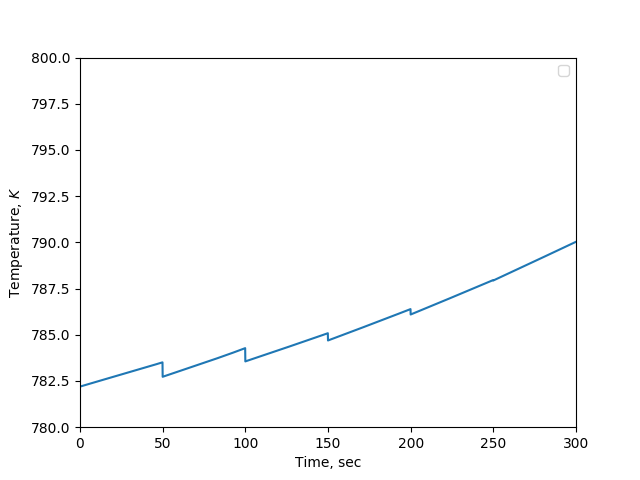
\includegraphics[width=\textwidth]{img1}
        \label{fig:img1}
    \end{minipage}
    \hfill
    \begin{minipage}[t]{0.49\textwidth}
        \centering
        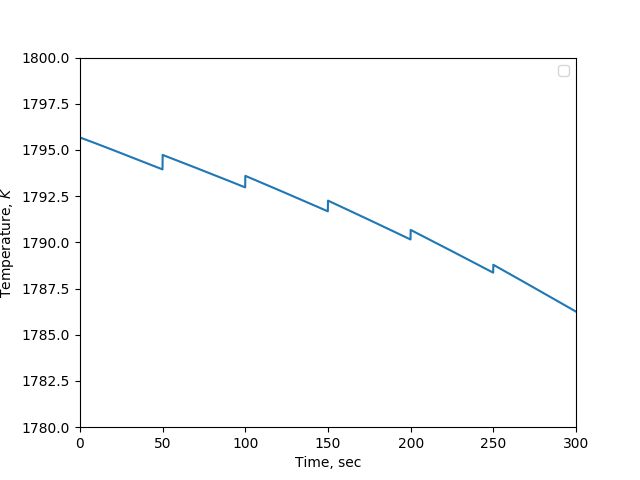
\includegraphics[width=\textwidth]{img2}
    \end{minipage}
    \caption {Температура воздуха в процессе нагрева и охлаждения на
    противоположном от точки подачи воздуха конце.}
\end{figure}

\begin{figure}[ht]
    \begin{minipage}[t]{0.49\textwidth}
        \centering
        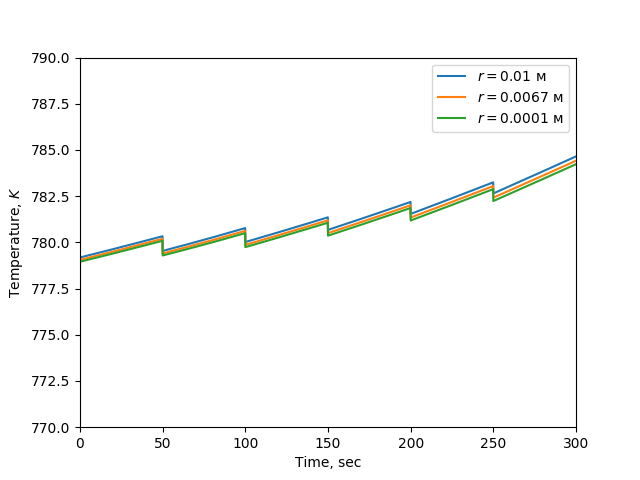
\includegraphics[width=\textwidth]{img3}
        \label{fig:img2}
    \end{minipage}
    \hfill
    \begin{minipage}[t]{0.49\textwidth}
        \centering
        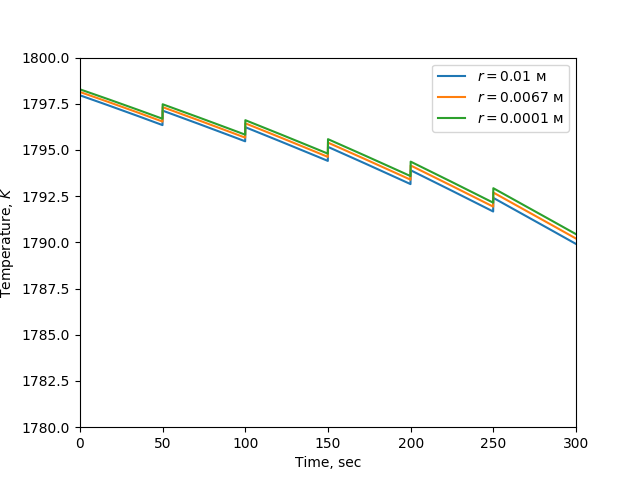
\includegraphics[width=\textwidth]{img4}
    \end{minipage}
    \caption {Температура керамики в процессе нагрева и охлаждения для
    различных слоев, от поверхности шара к его центру.}
\end{figure}

Необходимо отметить, что решаемая задача является весьма сложной для
методов МКР МКО и МКЭ. Она решается следующим образом. Задается
температура керамики в начальной стадии нагрева. Затем моделируются
многократно процессы нагрева и охлаждения керамики до тех пор, пока
температура в начале стадии нагрева не стабилизируется. 

При характерных для керамики значений коэффициентов
температуропроводности, рассмат риваемая система дифференциальных
уравнений является “жесткой”. Это требует задания малых характерных
размеров по пространственным координатам и по времени, что
обуславливает значительный расход вычислительных ресурсов. Применение
данного подхода существенно сокращает необходимые для решения задачи
ресурсы. 

\section{Заключение}

Анализ существующих методов решения систем дифференциальных уравнений
в частных производных, включая их достоинства и недостатки.

На основе анализа недостатков существующих методов предлагается
эффективный численный метод решения этих задач (метод контрольных
точек). Метод основан на сведении решения СДУЧП к решению задач
линейного программирования.

Метод иллюстрируется расчетом периодического теплообменника со
сферическим заполнением.

\begin{thebibliography}{999}
\bibitem{BZK2012} Бахвалов Н. С., Жидков Н. П., Кобельков Г. М.
    Численные методы. Учебник. – 2012.
\bibitem{KMP2018} Клер А. М., Маринченко А. Ю., Потанина Ю. М.
    Разработка математической модели системы высокотемпературных
    керамических теплообменников периодического действия
    //Известия Томского политехнического университета. Инжиниринг
    георесурсов. – 2018. – Т. 329. – №. 3. – С. 26-35.
\bibitem{KGS1970} Кошляков Н. С., Глинер Э. Б., Смирнов М. М.
    Уравнения в частных производных математической физики //М.:
    Высшая школа. – 1970. – Т. 712. – С. 11.
\bibitem{PS1970} Пантакар С., Сполдинг Д. Тепло и массообмен в
    пограничных слоях. – 1971.
\bibitem{SN1978} Самарский А. А., Николаев Е. С. Методы решения
    сеточных уравнений: Учебное пособие. – Наука. Гл. ред. физ.-мат.
        лит., 1978.
\bibitem{JG1961} Юдин Д. Б., Гольштейн Е. Г. Задачи и методы линейного
    программирования. – 1961.

\bibitem{C2020} Calatayud J. et al. Constructing reliable
    approximations of the probability density function to the random
    heat PDE via a finite difference scheme //Applied Numerical
    Mathematics. – 2020. – Т. 151. – С. 413-424.
\bibitem{CTO2018}Cebula A., Taler J., Ocłoń P. Heat flux and
    temperature determination in a cylindrical element with the use of
    Finite Volume Finite Element Method //International Journal of
    Thermal Sciences. – 2018. – Т. 127. – С. 142-157.
\bibitem{EGH2000}Eymard R., Gallouët T., Herbin R. Finite volume
    methods //Handbook of numerical analysis. – 2000. – Т. 7. – С.
    713-1018.
\bibitem{S1985} G. Smith, Numerical solution of partial differential
    equations: finite difference methods. Oxford university press, p.
    321, 1985.
\bibitem{G2007} Gale D. Linear programming and the simplex method
    //Notices of the AMS. – 2007. – Т. 54. – №. 3. – С. 364-369.
\bibitem{J2012} Johnson C. Numerical solution of partial differential
    equations by the finite element method. – Courier Corporation,
    2012.
\bibitem{KD2018}Kazem S., Dehghan M. Application of finite difference
    method of lines on the heat equation //Numerical Methods for
    Partial Differential Equations. – 2018. – Т. 34. – №. 2. – С.
    626-660.
\bibitem{ZTZ2005}Zienkiewicz O. C., Taylor R. L., Zhu J. Z. The finite
    element method: its basis and fundamentals. – Elsevier, 2005.
\end{thebibliography}

\begin{bibliographyl}{999}
\bibitem{KBZ2012} N. Bakhvalov, G. Kobelkov, N. Zhidkov. Numerical
    methods. Textbook. BINOM. Knowledge laboratory, 2012.

\bibitem{KMP2018}A. Kler, A. Marinchenko, Yu. Potanina "Development of
    a mathematical model of a system of high-temperature ceramic heat
    exchangers of periodic action." Bulletin of the Tomsk Polytechnic
    University. Georesource Engineering 329.3, 2018.

\bibitem{K1970}N. Koshlyakov, Partial differential equations of
    mathematical physics Higher school, Moscow p.712, 1970.
    
\bibitem{PS1968}S. Patankar, D. Spalding, Heat and mass transfer in
    boundary layers. Morgan-Grampian, 1968.

\bibitem{NS1978} A. Samarsky, E. Nikolaev, Methods for solving grid
    equations: textbook. for universities. The main editorial office
    of physical and mathematical literature of the Nauka publishing
    house. Moscow, p.528, 1978.

\bibitem{YH1961}D. Yudin, E. Holstein, Problems and Methods of Linear
    Programming, Soviet Radio. Moscow, p. 494, 1961.


\bibitem{C2020} Calatayud J. et al. Constructing reliable
    approximations of the probability density function to the random
    heat PDE via a finite difference scheme //Applied Numerical
    Mathematics. – 2020. – Т. 151. – С. 413-424.
\bibitem{CTO2018}Cebula A., Taler J., Ocłoń P. Heat flux and
    temperature determination in a cylindrical element with the use of
    Finite Volume Finite Element Method //International Journal of
    Thermal Sciences. – 2018. – Т. 127. – С. 142-157.
\bibitem{EGH2000}Eymard R., Gallouët T., Herbin R. Finite volume
    methods //Handbook of numerical analysis. – 2000. – Т. 7. – С.
    713-1018.
\bibitem{S1985} G. Smith, Numerical solution of partial differential
    equations: finite difference methods. Oxford university press, p.
    321, 1985.
\bibitem{G2007} Gale D. Linear programming and the simplex method
    //Notices of the AMS. – 2007. – Т. 54. – №. 3. – С. 364-369.
\bibitem{J2012} Johnson C. Numerical solution of partial differential
    equations by the finite element method. – Courier Corporation,
    2012.
\bibitem{KD2018}Kazem S., Dehghan M. Application of finite difference
    method of lines on the heat equation //Numerical Methods for
    Partial Differential Equations. – 2018. – Т. 34. – №. 2. – С.
    626-660.
\bibitem{ZTZ2005}Zienkiewicz O. C., Taylor R. L., Zhu J. Z. The finite
    element method: its basis and fundamentals. – Elsevier, 2005.
\end{bibliographyl}

\abth{% об авторах
\aboutauthors{%первый автор
    \textbf{Клер Александр Матвеевич}, д-р тех. наук, проф., Институт
    систем энергетики им. Л.А. Мелентьева СО РАН, 
    Иркутск, 664033, Российская Федерация, 
    email: kler@isem.irk.ru
   % doi https://orcid.org/xxxx-xxxx-xxxx-xxxx	
}{%
    \textbf{Aleksandr M. Kler}, Dr. Sci. (Technics), Prof.,
    Melentiev Energy Systems Institute SB RAS,
    Irkutsk, 664003, Russian Federation,
    kler@isem.irk.ru
 %\\https://orcid.org/xxxx-xxxx-xxxx-xxxx
}
\aboutauthors{%второй автор
    \textbf{Апанович Данил Владимирович}, аспирант, Институт систем
    энергетики им. Л.А. Мелентьева СО РАН, 
    Иркутск, 664033, Российская Федерация, 
    email: dvapan@gmail.com
   % doi https://orcid.org/xxxx-xxxx-xxxx-xxxx	
}{%
    \textbf{Danil V. Apanovich},Dr. Sci. (Technics), Prof.,
    Melentiev Energy Systems Institute SB RAS,
    Irkutsk, 664003, Russian Federation,
    email: dvapan@gmail.com
 }}


 \ra{26.07.2021}{26.09.2021}% не изменять


\end{article}
\end{document}
